\hypertarget{amk-methods}{%
\section{Methods}\label{amk-methods}}

This section describes the novel methods we developed to simulate the AK model including lattice generation, bond colouring and the inverse mapping between flux sector and gauge sector. Implementations are available online as a Python package called Koala (Kitaev On Amorphous LAttices)~\autocite{hodsonKoalaKitaevAmorphous2022}. All results and figures herein were generated with Koala.

\hypertarget{voronisation}{%
\subsection{Voronisation}\label{voronisation}}

\hypertarget{fig:lattice_construction_animated}{%
\begin{figure}
\centering
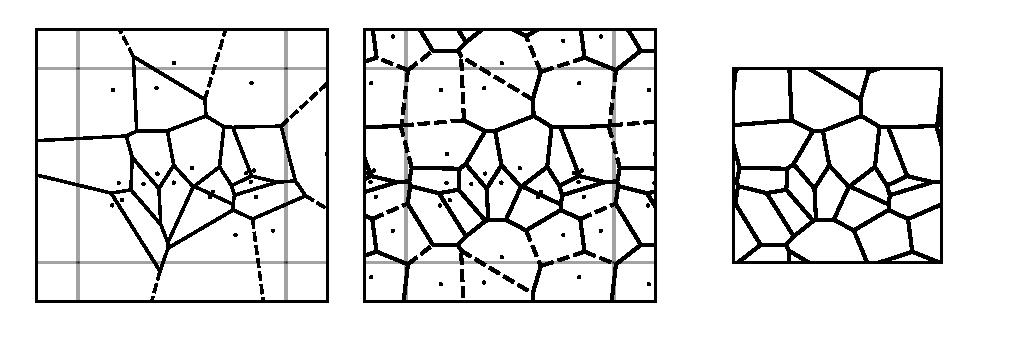
\includegraphics[width=1\textwidth,height=\textheight]{figure_code/amk_chapter/lattice_construction_animated/lattice_construction_animated}
\caption[{Lattice Construction}]{(Left) Lattice construction begins with the Voronoi partition of the plane with respect to a set of seed points (black points) sampled uniformly from \(\mathbb{R}^2\). (Center) However, we want the Voronoi partition of the torus, so we tile the seed points into a three by three grid. The boundaries of each tile are shown in light grey. (Right) Finally, we identify edges corresponding to each other across the boundaries to produce a graph on the torus. \href{http://thomashodson.com/assets/thesis/amk_chapter/lattice_construction_animated/lattice_construction_animated.gif}{ Animated version online.}}
\label{fig:lattice_construction_animated}
\end{figure}
}

The lattices we use are Voronoi partitions of the torus~\autocite{mitchellAmorphousTopologicalInsulators2018,marsalTopologicalWeaireThorpeModels2020,florescu_designer_2009}. We start by sampling \emph{seed points} uniformly (or otherwise) on the torus. As most off the shelf routines for computing Voronoi partitions are defined on the plane rather than the torus, we tile our seed points into a \(3\times3\) pr \(5\times5\) grid before calling a standard Voronoi routine~\autocite{barberQuickhullAlgorithmConvex1996} from the python package Scipy~\autocite{virtanenSciPyFundamentalAlgorithms2020}. Finally, we undo the tiling to the grid by identifying edges in the tiled lattice which are identical, yielding a trivalent lattice on the torus. We encode our lattices with edge lists \([(i,j), (j,k)\ldots]\) and an additional vector \((\{-1,0,+1\}, \{-1,0,+1\})\) for each edge that encodes the sense in which it crosses the periodic boundary conditions, equivalent to how the edge leaves the unit cell were the system to tile the plane, see \protect\hyperlink{app-lattice-generation}{appendix A.3} for more detail.

The graph generated by a Voronoi partition of a 2D surface is always planar. This means that no edges cross each other when the graph is embedded into the plane. It is also trivalent in that every vertex is connected to exactly three edges~\autocite{voronoiNouvellesApplicationsParamètres1908,watsonComputingNdimensionalDelaunay1981}.

\hypertarget{colouring-the-bonds}{%
\subsection{Colouring the Bonds}\label{colouring-the-bonds}}

\hypertarget{fig:multiple_colourings}{%
\begin{figure}
\centering
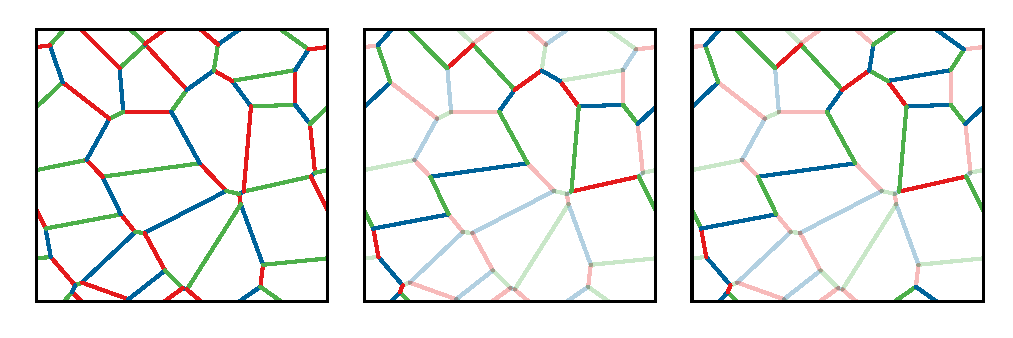
\includegraphics[width=1\textwidth,height=\textheight]{figure_code/amk_chapter/multiple_colourings/multiple_colourings}
\caption[{Colourings of an Amorphous Lattice}]{Different valid three-edge-colourings of an amorphous lattice. Colors that differ from the leftmost panel are highlighted in the other panels.}
\label{fig:multiple_colourings}
\end{figure}
}

To be solvable the AK model requires that each edge in the lattice be assigned a label \(x\), \(y\) or \(z\), such that each vertex has exactly one edge of each type connected to it. This problem must be distinguished from that considered by the famous four-colour theorem~\autocite{appelEveryPlanarMap1989}. The four-colour theorem is concerned with assigning colours to the \textbf{vertices} of planar graphs, such that no vertices that share an edge have the same colour. Here we are instead concerned with finding an edge colouring.

For a graph of maximum degree \(\Delta\), \(\Delta + 1\) colours are always enough to edge-colour it. An \(\mathcal{O}(mn)\) algorithm exists to do this for a graph with \(m\) edges and \(n\) vertices~\autocite{gEstimateChromaticClass1964}. Restricting ourselves to graphs with \(\Delta = 3\), these graphs are known as cubic graphs. Cubic graphs can be four-edge-coloured in linear time~\autocite{skulrattanakulchai4edgecoloringGraphsMaximum2002}. However we need a three-edge-colouring of our cubic graphs, which turns out to be more difficult. Cubic, planar, \emph{bridgeless} graphs can be three-edge-coloured if and only if they can be four-face-coloured~\autocite{tait1880remarks}. Bridges are edges that connect otherwise disconnected components. An \(\mathcal{O}(n^2)\) algorithm exists for these~\autocite{robertson1996efficiently}. However, it is not clear whether this extends to cubic, \textbf{toroidal} bridgeless graphs.

A four-face-colouring is equivalent to a four-vertex-colouring of the dual graph, see \protect\hyperlink{app-lattice-generation}{appendix A.3}. So if we could find a four-vertex-colouring of the dual graph we would be done. However vertex-colouring a toroidal graph may require up to seven colours~\autocite{heawoodMapColouringTheorems}! The complete graph of seven vertices \(K_7\) is a good example of a toroidal graph that requires seven colours.

Luckily, some problems are harder in theory than in practice. Three-edge-colouring cubic toroidal graphs appears to be one of those things. To find colourings, we use a Boolean Satisfiability Solver or SAT solver. A SAT problem is a set of statements about a set of boolean variables, such as ``\(x_1\) or not \(x_3\) is true''. A solution to a SAT problem is a assignment \(x_i \in {0,1}\) that satisfies all the statements~\autocite{Karp1972}. General purpose, high performance programs for solving SAT problems have been an area of active research for decades~\autocite{alounehComprehensiveStudyAnalysis2019}. Such programs are useful because, by the Cook-Levin theorem, any NP problem can be encoded (in polynomial time) as an instance of a SAT problem . This property is what makes SAT one of the subset of NP problems called NP-Complete~\autocite{cookComplexityTheoremprovingProcedures1971,levin1973universal}. Thus, it is a relatively standard technique in the computer science community to solve NP problems by first transforming them to SAT instances and then using an off the shelf SAT solver. The output of this can then be mapped back to the original problem domain.

Whether graph colouring problems are in NP or P seems to depend delicately on the class of graphs considered, the maximum degree and the number of colours used. Since we I didn't know of any better algorithm for the problem at hand using a SAT solver appeared to be a reasonable first method to try and it turns out to be fast enough in practice that it is by no means to rate limiting step for solving instances of our model. In \protect\hyperlink{app-lattice-generation}{appendix A.3} I detail the specifics of how I mapped edge-colouring problems to SAT instances and show a breakdown of where the computational effort is spent, the majority being on diagonalisation.

\hypertarget{mapping-between-flux-sectors-and-bond-sectors}{%
\subsection{Mapping between flux sectors and bond sectors}\label{mapping-between-flux-sectors-and-bond-sectors}}

\hypertarget{fig:flux_finding}{%
\begin{figure}
\centering
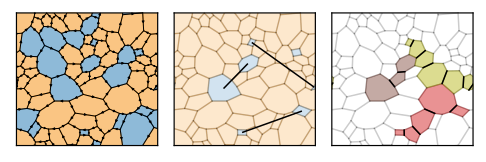
\includegraphics[width=1\textwidth,height=\textheight]{figure_code/amk_chapter/flux_finding/flux_finding}
\caption[{Finding Bond Sectors from Flux Sectors}]{(Left) The ground state flux sector and bond sector for an amorphous lattice. Bond arrows indicate the direction in which \(u_{jk} = +1\). Plaquettes are coloured blue when \(\hat{\phi}_i = -1\) (\(-i\)) for even/odd plaquettes and orange when \(\hat{\phi}_i = +1\) (\(+i\)) for even/odd plaquettes. (Centre) To transform this to the target flux sector (all \(+1\)/\(+i\)), we first flip any \(u_{jk}\) that are between two fluxes. This leaves a set of isolated fluxes that must be annihilated. Then, these are paired up as indicated by the black lines. (Right) A* search is used to find paths (coloured plaquettes) on the dual lattice between each pair of fluxes and the corresponding \(u_{jk}\) (shown in black) are flipped. One flux will remain because the starting and target flux sectors differed by an odd number of fluxes.}
\label{fig:flux_finding}
\end{figure}
}

In the AK model, going from the bond sector to flux sector is done simply from the definition of the fluxes

\[ \phi_i = \prod_{(j,k) \; \in \; \partial \phi_i} i u_{jk}.\]

The reverse, constructing the bond sector \(\{u_{jk}\}\) that corresponds to a particular flux sector \(\{\{\Phi_i\}\) is not so trivial. The algorithm, shown visually in \cref{fig:flux_finding} is this:

\begin{enumerate}
\def\labelenumi{\arabic{enumi}.}
\item
  Fix the gauge by choosing some arbitrary \(u_{jk}\) configuration. In practice, we use \(u_{jk} = +1\). This chooses an arbitrary one of the four topological sectors.
\item
  Compute the current flux configuration and how it differs from the target one. Consider any plaquette that differs from the target as a defect.
\item
  Find any adjacent pairs of defects and flip the \(u_jk\) between them. This leaves a set of isolated defects.
\item
  Pair the defects up using a greedy algorithm and compute paths along the dual lattice between each pair of plaquettes using A*. Flipping the corresponding set of bonds transports one flux to the other and annihilates both.
\end{enumerate}
